%% LyX 2.0.6 created this file.  For more info, see http://www.lyx.org/.
%% Do not edit unless you really know what you are doing.
\documentclass[letterpaper]{article}
\usepackage[latin9]{inputenc}
\usepackage{url}
\usepackage{amsmath}
\usepackage{amssymb}
\usepackage{graphicx}
\usepackage{setspace}
\usepackage[authoryear]{natbib}
\onehalfspacing

\makeatletter

%%%%%%%%%%%%%%%%%%%%%%%%%%%%%% LyX specific LaTeX commands.
\pdfpageheight\paperheight
\pdfpagewidth\paperwidth


%%%%%%%%%%%%%%%%%%%%%%%%%%%%%% User specified LaTeX commands.

%\setlength{\parindent}{0in}
\setlength{\textheight}{8.9in}
\setlength{\textwidth}{6.8in}
\setlength{\oddsidemargin}{-0.3in}
\setlength{\evensidemargin}{0.0in}
\addtolength{\topmargin}{-1in}


\usepackage{amsfonts}\usepackage{caption}\usepackage{subcaption}

\usepackage{url}\usepackage{multirow}

\newcommand{\bmeta}{\boldsymbol{\eta}}
\newcommand{\bmtheta}{\boldsymbol{\theta}}
\newcommand{\bmbeta}{\boldsymbol{\beta}}
\newcommand{\bmphi}{\boldsymbol{\phi}}
\newcommand{\bmpi}{\boldsymbol{\pi}}
\newcommand{\bmxi}{\boldsymbol{\xi}}
\newcommand{\bmnu}{\boldsymbol{\nu}}
\newcommand{\bmmu}{\boldsymbol{\mu}}
\newcommand{\bmalpha}{\boldsymbol{\alpha}}
\newcommand{\bmzeta}{\boldsymbol{\zeta}}
\newcommand{\bmgamma}{\boldsymbol{\gamma}}
\newcommand{\bmomega}{\boldsymbol{\omega}}

\newcommand{\bmY}{\mathbf{Y}}
\newcommand{\bmZ}{\mathbf{Z}}
\newcommand{\bmX}{\mathbf{X}}
\newcommand{\bmV}{\mathbf{V}}
\newcommand{\bmW}{\mathbf{W}}
\newcommand{\bmU}{\mathbf{U}}
\newcommand{\bmR}{\mathbf{R}}
\newcommand{\bmS}{\mathbf{S}}
\newcommand{\bmb}{\mathbf{b}}

\newcommand{\bmM}{\mathbf{M}}
\newcommand{\bmSigma}{\boldsymbol{\Sigma}}
\newcommand{\bmI}{\mathbf{I}}
\newcommand{\bmTheta}{\boldsymbol{\Theta}}

 


\newcommand{\mydots}{...}

\usepackage{color}\usepackage{xcolor}

\definecolor{mygreen}{rgb}{0,0.75,0}
\definecolor{mypurple}{rgb}{0.7,0,0.8}

\newcommand{\shade}[1]{\colorbox{gray}{#1}}
%\newcommand{\highlight}[1]{\colorbox{yellow}{#1}}
\newcommand{\gbox}[1]{\colorbox{green}{#1}}
\newcommand{\tcr}[1]{\textcolor{red}{#1}}
\newcommand{\tcg}[1]{\textcolor{mygreen}{#1}}
\newcommand{\highlight}[1]{\textcolor{blue}{#1}}
\newcommand{\tcp}[1]{\textcolor{mypurple}{#1}}
\newcommand{\tcbk}[1]{\textcolor{black}{#1}}

\makeatother

\begin{document}

\title{Technical Report: Fast Updating for Bayesian Joint Hierarchical Model for Prediction of Latent Health States}


\author{ Aaron J Fisher, R Yates Coley, Scott L Zeger}


\date{\today}

\maketitle

\section*{Abstract}

This technical report presents an importance sampling algorithm for rapidly obtaining updated individualized predictions for the Bayesian joint model proposed in \citet{coley2015prostateSurvaillence}. Algorithm details are given and performance is assessed. Data and code are available at \url{http://github.com/rycoley/XXX}.

\smallskip{}



\section*{Introduction}

Heirarchical bayes models can be especially useful in the context of precision medicine, when scientists are interested not only in estimating treatment effects, but also in estimating the risk for any individual patient. In the context of heirarchical models, treatment effects can be estimated from population-level parameters, and the risk for any specific patient can be described by a patient-level latent class. For example, \citet{coley2015prostateSurvaillence} use a patient specific latent class to identify patients as having either benign cancer, or aggressive cancer. In a bayesian setting, estimation at both levels of the model, the population level and the patient level, can be done by averaging over the posterior. When such models are fit on a training dataset using Markov Chain Monte Carlo (MCMC), risk estimates are immediately available for any patient in the training dataset. 

A computational challenge arises though when new patients enter the clinic, or when existing patients accrue new measurements. Here, clinicians may wish to give patients a fast, in-visit estimate of their risk. However, traditional MCMC approaches for new risk estimates require refitting the entire model, which can take hours to complete.

In this technical report we describe how importance sampling (IS) can instead be used in precision medicine settings to get fast risk estimates in response to new patient data. We apply this to a version of the prostate cancer model proposed by \citet{coley2015prostateSurvaillence} to get fast risk estimates for new, simulated patients. This approach can be combined with periodic refitting of the entire model via MCMC, in order to update estimates of the population-level parameters \citep{Lee2002}.

This IS approach is related to online learning methods, which aim to continuously update population-level parameters at a constant computational cost over time. We avoid a fully online approach though, due to additional known challenges in online learning. Specifically, our use of IS can be viewed as a 1-step version of a sequential importance sampler (SIS), also known as particle filter. Employing a generic particle filter to get updated estimates of the population parameters would seem to be a natural extension, but particle filters are known to suffer from the problem of degeneracy in the precense of ``static'' parameters (see section II of \citet{Andrieu2005} for an intuitive explanation). This applies in our case, where the population-level parameters are modeled as static, and changing as more data is acquired. A combination of IS and periodic MCMC \citep{Lee2002} can be used to update population-level posteriors, but is not fully online as the computational cost of each MCMC iteration increases as more data is acquired.

Online, or streaming, model fitting has been explored in the literature on topic modeling for corpuses of texts. Text corpuses are often too large to fit an entire model on at once, making online fitting a more feasible option. For example, \citet{hoffman2010online_variational_bayes_LDA_text_analysis} propose a online variational bayes approach for topic modeling. Our specific context within personalized medicine is different in that while the model may be complex and contain several layes, the data can be fully stored in memory at once. Thus, while the approach of combining IS with periodic MCMC is not fully online, and not feasible for topic modeling, it is still a feasible option for limited sample sizes in our problem. An additional benefit of IS, in contrast to variational bayes approaches, is that the formulas required to apply IS are simple to derive, and can be easily ported to other applications within precision medicine.


\section{Introduction}

\citet{coley2015prostateSurvaillence} presents a Bayesian joint hierarchical model for predicting a latent health state from longitudinal clinical measurements. Model development was motivated by an application to active surveillance of low risk prostate cancer. Previous joint latent class modeling approaches (e.g., \citet{Lin2002}) are unsuitable for this context as they do not accommodate measurement error-- specifically, cancer state determinations based on biopsied tissue are prone to misclassification-- nor do they allow for observations to be missing not at random \citep{Little2014}. The proposed model addresses these limitations, enabling estimation of an individual's underlying prostate cancer state. These individualization predictions can then be communicated to clinicians and patients to inform decision making.

For this prediction model to be most useful in a clinical setting, however, it is necessary to be able to update posterior estimates quickly to incorporate new biopsy or PSA results during a patient's visit. This precludes re-running the full MCMC to obtain updated posteriors of patient-specific variables. Instead, we use importance sampling \citep{Bishop2006} to obtain rapid prediction updates. Using posterior estimates obtained from current data, the proposed importance sampling algorithm updates these estimates for either a new patient or new data on an existing patient in a matter of seconds.

Many options exist for performing online updating of Bayesian models. We chose to use an importance sampling approach because... \citep{Geweke1989}.

In this this technical report, we first provide an overview of the latent class prediction model before detailing the importance sampling algorithm we have developed for enabling real-time updates. Next, we will apply the proposed algorithm to simulated data and compare predictions to those obtained by full MCMC runs. Finally, we close with a discussion of future research.


\section{Bayesian Joint Hierarchical Latent Class Model}

In this section, we briefly summarize the joint model proposed in \citet{coley2015prostateSurvaillence} for predicting latent cancer state for men participating in Active Surveillance for low risk prostate disease. Predictions are made by incorporating information from repeated prostate specific antigen (PSA) and biopsy measurements for all individuals, as well as true cancer state information observed in a subset of the cohort. In this technical report, we will focus on the model that assumes biopsy and latent class observation are missing at random, that is, not associated with the latent state after conditioning on observed clinical variables. For more model details and application background, please see \citet{coley2015prostateSurvaillence}.

Let $\eta_{i}$ indicate the true cancer state for individual $i$, $i=1,\dots,n$, defined using the the Gleason score \citep{Gleason1977,Gleason1992} that would be assigned if his entire prostate were to be removed and pathologic analysis performed: $\eta_{i}=0$ if Gleason $\leq$ 6 or \textit{indolent} and $\eta_{i}=1$ if Gleason $\geq$ 7 or \textit{aggressive}. True cancer state then follows a Bernoulli distribution-- $\eta_{i}\sim Bernoulli(\rho)$-- where we assume here, for simplicity, a shared underlying probability of aggressive cancer, $\rho$. This true cancer state is observed in a subset of patients who choose to have their prostate surgically removed; as such, $\eta_{i}$ is a partially latent variable.

Next, define the following mixed effects model \citep{Laird1982} for an individual's PSA over time where mean effects for predictors are allowed to vary across groups defined by the partially latent true cancer state: 
\begin{eqnarray*}
\big[\, Y_{im}|\eta_{i}=k,\bmX_{im},\bmZ_{im}\,\big]=\bmX_{im}\bmbeta+\bmZ_{im}\bmb_{i}+\epsilon_{im}
\end{eqnarray*}
where $Y_{im}$ is the observed (log-transformed) PSA, $\bmX_{im}$ and $\bmZ_{im}$ are vectors of covariates for individual $i$'s $m$th PSA measurement, $\bmbeta$ is a parameter vector for fixed effects, and $\bmb_{i}$ is the patient-specific vector of random effects. Following the specification of a Bayesian mixed effects model presented by Gelman and Hill (2006)\nocite{Gelman2006}, unscaled random effects are centered at the mean effects for each latent class $k$, $\bmmu_{k}$: 
\begin{eqnarray*}
\big[\check{\bmb_{i}}|\eta_{i}=k\big]\sim MVN(\bmmu_{k},\Sigma_{k}),\quad k=0,1
\end{eqnarray*}
where $\Sigma_{k}$ is a covariance matrix that allows for correlation between random effects. Random effects are then scaled with parameter vector $\bmxi$: $\bmb_{i}=diag(\check{\bmb_{i}}\bmxi^{T})$. Lastly, residuals $\epsilon_{im}$ are assumed to follow a normal distribution with mean 0 and variance $\sigma^{2}$.

Finally, let $(B_{ij},R_{ij})$ denote binary variables for individual $i$ in annual interval $j$ indicating, respectively, whether a biopsy was performed and, when it was, if \textit{reclassification} was observed, i.e. a determination of Gleason $\geq$ 7 made. $(B_{ij},R_{ij})$ is defined for $j=1,\dots,J_{i}$ where $J_{i}$ is the time of reclassification or censoring for patient $i$. For each time interval with a biopsy, $B_{ij}=1$, we use logistic regression to model its result conditional on true cancer state: 
\begin{eqnarray}
P(R_{ij}=1|B_{ij}=1,\eta_{i}=k,\bmV_{ij},\bmgamma)=\text{logit}^{-1}\big(\bmV_{ij}(k)\bmgamma\big)\label{eq:p_rc}
\end{eqnarray}
where $\bmV_{ij}(k)$ is a matrix of time-varying predictors including $\eta_{i}$ and $\bmgamma$ is a parameter vector.

We then define the joint probability of the parameters given data and unobserved latent variables: 
\begin{eqnarray}
 &  & L\Big(\rho,\bmbeta,(\bmmu_{k},\Sigma_{k}),\bmgamma\,|\,\big(\eta_{i},(\bmY_{i},\bmb_{i},\underline{\bmX_{i}},\underline{\bmZ_{i}}),(\mathbf{B}_{i},\mathbf{R}_{i},\underline{\bmV_{i}})\big),i=1,\mydots,n\Big)\nonumber \\
 &  & \quad=\prod_{i=1}^{n}\,\rho^{\eta_{i}}\,(1-\rho)^{1-\eta_{i}}\, f(\bmY_{i}|\eta_{i},\underline{\bmX_{i}},\underline{\bmZ_{i}},\bmb_{i},\bmbeta,\sigma^{2})\, g(\bmb_{i}|\bmmu_{\eta_{i}},\Sigma_{\eta_{i}})\nonumber \\
 &  & \qquad\qquad\prod_{j=1}^{J_{i}}\big(P(R_{ij}=1|\eta_{i},\bmV_{ij},\bmgamma)^{R_{ij}}P(R_{ij}=0|\eta_{i},\bmV_{ij},\bmgamma)^{1-R_{ij}}\big)^{B_{ij}}\label{eq:lik-inf}
\end{eqnarray}
where $f$ and $g$ are multivariate normal densities for the vector of log-transformed PSAs $\bmY_{i}$, and random effects $\bmb_{i}$, respectively, each with mean and covariance as defined above, given covariance matrices $\underline{\bmX_{i}}=[X_{i1},\dots,X_{iM_{i}}]$ and $\underline{\bmZ_{i}}=[Z_{i1},\dots,Z_{iM_{i}}]$. $\mathbf{B}_{i},\mathbf{R}_{i}$ represent vectors for biopsy and reclassification for individual $i$ with associated covariance matrix $\underline{\bmV_{i}}$.

Bayesian methods are used to identify posteriors for model parameters and latent variables. Discussion of prior specification can be found in \citet{coley2015prostateSurvaillence}. After specifying priors for all model parameters, the join posterior distribution of the parameter and latent variables is: 
\begin{eqnarray}
 &  & p\Big(\rho,\bmbeta,(\bmmu_{k},\Sigma_{k}),\bmgamma,(\eta_{i},\bmb_{i})\,|\,\big((\bmY_{i},\underline{\bmX_{i}},\underline{\bmZ_{i}}),(\mathbf{B}_{i},\mathbf{R}_{i},\underline{\bmV_{i}})\big);\bmTheta\Big)\nonumber \\
 &  & \qquad\propto L\Big(\rho,\bmbeta,(\bmmu_{k},\Sigma_{k}),\bmgamma\,|\,\big(\eta_{i},(\bmY_{i},\bmb_{i},\underline{\bmX_{i}},\underline{\bmZ_{i}},(\mathbf{B}_{i},\mathbf{R}_{i},\underline{\bmV_{i}})\big)\Big)\times\bmpi\big(\rho,\bmbeta,(\bmmu_{k},\Sigma_{k}),\bmgamma|\bmTheta\big)\label{eq:post-inf}
\end{eqnarray}
where $\bmpi(\cdot|\bmTheta)$ denotes the joint prior density for model parameters with hyperparameters $\bmTheta$ with indexing on $i,\, j,$ and $k$ suppressed for clarity in presentation.


\section{Importance Sampling Algorithm for Fast Prediction Updates}

Next, we detail an importance sampling algorithm that enables rapid updates of joint latent class model predictions. To simplify presentation, we abbreviate notation for the joint posterior given above in Equation \ref{eq:post-inf}: 
\begin{equation}
p(\theta,b_{1:n}|y_{1:n})\propto\prod_{i=1}^{n}[f(y_{i}|b_{i},\theta)g(b_{i}|\theta)]\pi(\theta)\label{eq:posterior_n}
\end{equation}
where $y_{i}$ is the vector of clinical measurements (PSA and biopsy) for patient $i$, $y_{1:n}$ is the list of measurements for the first $n$ patients, $b_{i}$ is a vector of latent variables (latent class and random effects) for patient $i$, $b_{1:n}$ is a list of latent variables for the first $n$ patients, $\theta$ contains the population-level parameters, $\pi$ is the prior for $\theta$, and $f$ and $g$ are multivariate distributions coming from the model likelihood in Equation \ref{eq:lik-inf}.

After posterior samples from the joint model are obtained for current data, importance sampling to update these estimates given new data requires three steps: first, generating proposal values for the latent variables to be updated, second, calculating weights for proposed values, and, third, weighting proposed values to estimate an updated posterior. We first illustrate how this process can be used to quickly estimate latent variables for a new patient before showing how similar calculations can be done to incorporate newly measured data on existing patients in real-time.

For a new patient (indexed by $i=n+1$), obtaining posterior predictions of latent variables requires calculating expectations with respect to the posterior distribution based on all $n+1$ patients (i.e. $p(\theta,b_{1:(n+1)}|y_{1:(n+1)})$). While we cannot immediately draw from this distribution, we can evaluate a function that is proportional to its density (Equation \ref{eq:posterior_n}). The posterior distribution based on the first $n$ patients provides an appropriate proposal distribution ($q$) from which to generate candidate values of $(\theta,b_{1:(n+1)})$: 
\begin{eqnarray*}
q(\theta,b_{1:(n+1)}) & := & g(b_{n+1}|\theta)p(\theta,b_{1:n}|y_{1:n})
\end{eqnarray*}


This approach is analogous to a one-step particle filter \citet{Bishop2006} and, practically, consists of taking $J$ draws of $\theta$ and $b_{1:n}$ from the previously fitted posterior in Equation \ref{eq:posterior_n}. Then, conditional on $\theta$, we draw $b_{n+1}$ from the distribution $g$. We index each of the resulting draws as $(\theta^{(j)},b_{1:(n+1)}^{(j)})$, with $j=1,\dots,J$. The importance weights $w_{j}$ are then proportional to 
\begin{eqnarray}
w^{(j)} & \propto & \frac{p(\theta^{(j)},b_{1:(n+1)}^{(j)}|y_{1:(n+1)})}{q(\theta^{(j)},b_{1:(n+1)}^{(j)})}\nonumber \\
 & \propto & \frac{\prod_{i=1}^{n+1}[f(y_{i}|b_{i}^{(j)},\theta^{(j)})g(b_{i}^{(j)}|\theta^{(j)})]\pi(\theta^{(j)})}{g(b_{n+1}^{(j)}|\theta^{(j)})\prod_{i=1}^{n}[f(y_{i}|b_{i}^{(j)},\theta^{(j)})g(b_{i}|\theta^{(j)})]\pi(\theta^{(j)})}\nonumber \\
 & = & f(y_{i}|b_{i}^{(j)},\theta^{(j)})\label{eq:importance-weights}
\end{eqnarray}


The final weights $w^{(j)}$ are standardized to sum to 1. The new posterior for $(\theta,b_{1:(n+1)})$ can then be represented as the mixture distribution satisfying $P(\theta=\theta^{(j)},b_{1:(n+1)}=b_{1:(n+1)}^{(j)})=w^{(j)}$. A posterior mean for $b_{(n+1)}$ can be calculated as $\sum_{j=1}^{J}w^{(j)}b_{(n+1)}^{(j)}$. The unstandardized weights can also be used in a rejection sampling procedure, although we found this approach to be less computationally efficient than importance sampling for our scenario.

For a patient $k$ with existing data, where we already have a posterior sample for their latent variable values, we instead use this posterior as our proposal distribution $q(\theta^{(j)},b_{1:n}^{(j)})$, with $i\leq n$. Let $y_{1:n}^{k+}$ refer to the data set after incorporating new data on patient $k$, where $y_{i}^{+}=y_{i}$ if $k\neq i$. The importance weights in Equation \ref{eq:importance-weights} then simplify to 
\begin{eqnarray*}
w^{(j)} & \propto & \frac{p(\theta^{(j)},b_{1:n}^{(j)}|y_{1:n}^{+})}{q(\theta^{(j)},b_{1:n}^{(j)})}\\
 & \propto & \frac{\prod_{i=1}^{n}[f(\ensuremath{y_{i}^{+}}|b_{i}^{(j)},\theta^{(j)})g(b_{i}^{(j)}|\theta^{(j)})]\pi(\theta^{(j)})}{\prod_{i=1}^{n}[f(\ensuremath{y_{i}}|b_{i}^{(j)},\theta^{(j)})g(b_{i}^{(j)}|\theta^{(j)})]\pi(\theta^{(j)})}\\
 & = & \frac{f(\ensuremath{y_{k}^{+}}|b_{k}^{(j)},\theta^{(j)})}{f(\ensuremath{y_{k}}|b_{k}^{(j)},\theta^{(j)})}
\end{eqnarray*}


Let $L_{k}$ denote that number of measurements for which we've previously fit a posterior for $b_{k}$, and let $N_{k}$ denote the number of new measurements we wish to incorporate into this posterior. Then, $y_{k}^{+}$ can be expressed as the vector $y_{k}^{+}=(y_{k[1]},y_{k[2]},\dots y_{k[L_{k}]},y_{k[L_{k}+1]}^{+},\dots y_{k[L_{k}+N_{k}]}^{+})$, where $y_{k[l]}^{+}$ is the $l^{th}$ measurement from patient $k$. If the repeated measures for each patient are independent conditional on $b_{i}$, as is the case in the proposed model, then the above ratio reduces to

\begin{eqnarray*}
w^{(j)} & \propto & \frac{\prod_{l=1}^{L_{k}+N_{k}}f(\ensuremath{y_{k[l]}^{+}}|b_{k}^{(j)},\theta^{(j)})}{\prod_{l=1}^{L_{i}}f(\ensuremath{y_{k[l]}}|b_{k}^{(j)},\theta^{(j)})}\\
 & = & \prod_{l=L_{k}+1}^{L_{k}+N_{k}}f(\ensuremath{y_{k[l]}^{+}}|b_{k}^{(j)},\theta^{(j)})
\end{eqnarray*}
We then proceed as above to get a re-weighted posterior for the latent variables of patient $k$.

For implementation in clinical practice, proposals for new patients can be re-generated prior to actually observing new data, so that only weight calculating and re-weighting of the proposal distribution needs to be done in real-time. Then, predictions for each patient can be obtained in a matter of seconds. By random chance, some patients will have data such that very few of the pre-generated proposed latent values will receive high weights; this can cause instability in posterior means. However, such scenarios can be detected by monitoring the effective size of the posterior sample, also known as the effective number of particles. When this number drops below a pre-specified threshold (e.g., 500), the procedure can be repeated with a larger set of pre-generated proposals.


\section{Application}

We assessed performance of the proposed importance sampling approach in a simulated dataset. We compared the posterior probability of latent class membership (specifically, $P(\eta_{i}=1)$) obtained from MCMC performed in \texttt{RJAGS} to the predictions obtained by the proposed importance sampling algorithm for each patient for whom true state was not observed. Agreement was examined for the new patient scenario, that is, proposal values for an individual's latent state were generated from population-level parameters and all his available data was used to calculate sampling weights. Code for simulating data and obtaining estimates is available at \texttt{http://github.com/rycoley/XXX}.

Results of this comparison are shown in Figure \ref{fig:jags-vs-pf}. Agreement between methods for newly introduced patients is strong; correlation between posterior probabilities from \texttt{JAGS} and the importance sampler is 0.XX. These findings indicate that the proposed importance sampling algorithm is an appropriate substitute for full MCMC runs in order to provide real-time updates in a clinical setting.

\begin{figure}
\centering{}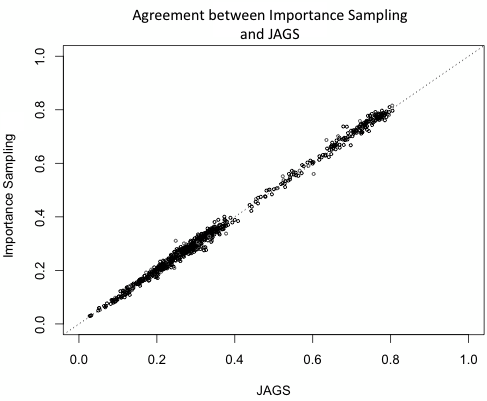
\includegraphics[width=0.7\textwidth]{2015-07-01_compare_fits_manual-edit} \caption{Agreement between importance sampling and JAGS posterior predictions of aggressive prostate cancer state for a new patient. (Dashed line indicates the axis of equality, i.e., perfect agreement.)\label{fig:jags-vs-pf} }
\end{figure}


Effective sample size...


\section{Conclusion}

The joint model of \citet{coley2015prostateSurvaillence} is among a growing number of statistical models for making individualized health predictions and recommendations. Development of such \textit{precision medicine} methods must occur within a framework for clinical implementation. Specifically, concerns about convenience, security, and effective communication must be addressed alongside statistical considerations. In this technical report, we have presented an importance sampling algorithm for obtaining fast predictions of latent health state based on the joint modeling framework of \citet{coley2015prostateSurvaillence}. This approach informs decision-making by enabling doctors and patients to access updated predictions in real-time in a clinical setting.

The proposed importance sampling approach still requires the periodic use of MCMC to perform full model updates, similar to the procedure described in Lee and Chia (2002)\nocite{Lee2002}. While fully online updating of all posteriors (that is, updating not dependent on periodic MCMC) via sequential importance resampling would be ideal, such online methods are known to suffer from the problem of degeneracy when the model includes static parameters (such as the population-level parameters in our model), as explained in Andrieu et al. (2005, section II)\nocite{Andrieu2005}.

\bibliographystyle{apalike}
\bibliography{inhealth-bib}

\end{document}
